\documentclass[12pt]{article}
\usepackage[utf8]{inputenc}
\usepackage[T1]{fontenc}
\usepackage{lmodern}
\usepackage{graphicx}
\usepackage[small]{caption}
\usepackage{amsmath, amssymb}
\usepackage{fullpage}
\usepackage{hyperref}
\newcommand{\R}{\mathbb{R}}
\newcommand{\Z}{\mathbb{Z}}
% helper macro for vectors
\usepackage{bm}
\newcommand{\vb}[1]{\ensuremath{\boldsymbol #1}}

\newtheorem{theorem}{Theorem}
\newtheorem{definition}{Definition}

\begin{document}
\author{Antoine Levitt}
\title{Finite volumes method for incompressible Navier-Stokes equations}
\maketitle
\abstract{
  In this project we study numerical methods to numerically approximate
the steady state of a flow. We present the Navier-Stokes equations and
their approximations for free convection (Boussinesq hypothesis). We
use the colocated scheme introduced in
\cite{che-09-col,che-08-col,che-06-num} and apply it to a benchmark
problem, a heated chimney. On this problem, different boundary
conditions are compared, and numerical properties of the scheme are
obtained.}
\newpage
\tableofcontents
\newpage

\section{Introduction}
The Navier-Stokes equations, discovered in the 19th century, are a
system of non-linear partial differential equations (PDEs) describing
the motion of fluid. These equations couple velocities, pressure and
other variables as required by the application field (temperature,
electrical charge and currents \dots), in which case the Navier-Stokes
are complemented by other equations, such as conservation laws for
temperature or Maxwell laws for electromagnetism. Due to their wide
applicability, they are essential for engineering. There is also a
number of open problems in the mathematical study of these
equations. In particular, the question of existence and smoothness of
solutions is one of the Millenium Prize Problems.

Fast, accurate and reliable numerical solutions to these equations is
an important goal for engineering. Reflecting this, many commercial
and research codes have been developed. Most of them belong to the
three classes of finite volume, finite element and finite difference
methods :

\begin{itemize}
\item {\bf Finite difference method} approximates fields by their
  values on points, and interpolates derivatives. This, while the
  simplest of all methods, generally yields poor accuracy.

\item {\bf Finite element method} convert the PDE into an equivalent
  variational form, then approximate the infinite-dimensional solution
  space by a finite-dimensional one, in which the variational problem
  can be solved.

\item {\bf Finite volume method} use Green formulas to convert the
  equation into a per-cell conservation equation. Fluxes are then
  interpolated from values at neighbouring cells.
\end{itemize}

All these methods discretize the solution according to a grid. There
are various choices for the location of the unknowns inside the grid,
and methods can be split between {\bf collocated} and {\bf staggered}
grids. In collocated grids, all variables are stored in the cell
centers. In staggered grids, scalar variables are still stored in cell
centers, but velocities are located at cell faces. The main motivation
for using staggered grids is to avoid the so-called checkerboard
pressure modes that arise from the discretization of first derivatives
in collocated grids.

Examples of classical schemes on staggered grids include the
Marker-And-Cell (MAC) scheme
\cite{har-65-num,Pat-80-num,har-65-num,nic-92-ana,cho-97-ana,cho-97-mac}. Collocated
grids need stabilisation to avoid checkerboard modes. Various methods
exist. We use a variant of the Brezzi-Pitk{\"a}ranta approach
\cite{mat-97-apr,brezzip,brezzip2}, which consists in introducing an
artificial diffusion term in the mass conservation equation.

Various scheme also exist to decouple the equations, most notably
variants of the projection method \cite{mat-97-pre}. This method,
valid only for transient analysis (which means steady state has to be
found as a limit of the transient process, while for other methods it
can be directly computed), uses a two-step algorithm to decouple
velocities and pressure, which greatly reduces computation time. The
SIMPLE algorithm is the most popular of these variants. However, these
methods need artificial boundary conditions for pressure, and can
cause artificial boundary layers to appear.

The algorithm we use is a fully implicit, fully coupled, collocated
finite volume scheme introduced by E. Chénier and R. Eymard
\cite{che-09-col,che-08-col,che-06-num}.

To test the accuracy of these variants in the context of free
convection (where fluid flow is only a result of temperature
gradients), G. Desrayaud organised a benchmark in 2007, around a
simple problem. TODOFIN : qu'est ce qu'on en fait, décrire les différents
codes.

% points \`a mentionner dans l'introduction:

% - passer en revue les m\'ethodes num\'eriques pour convection naturelle:

% sch\'emas \'el\'ements finis \cite{gun-89-fin,pironneau}, 
% volumes finis sur grilles d\'ecal\'ees, sch\'ema MAC \cite{har-65-num,Pat-80-num},
% \'etudi\'e dans \cite{har-65-num,nic-92-ana,cho-97-ana,cho-97-mac}
% volumes finis  colocalis\'es (collocated), n\'ecessitent stabilisation
% \cite{mat-97-apr,brezzip,brezzip2}

% m\'ethodes de projection (solution stationnaire n\'ecessite limite
% probl\`eme transitoire, et conditions aux limites
% artificielles en pression) \cite{mat-97-pre} 

% m\'ethodes coupl\'ees pour pb stationnaires ou transitoires
%  (mais nonlin\'earit\'es impliquent Newton ou limite pb transitoire) 



% - benchmark pour comparer diff\'erentes approches en convection naturelle

% - ranger les diff\'erents logiciels du bench selon les m\'ethodes num\'eriques
% utilis\'ees

% FLUENT \cite{mat-97-apr,mat-97-pre}

% code colocalis\'e Ch\'enier \cite{che-09-col,che-08-col,che-06-num}

% AQUILON devenu THETIS

\section{Physical context}
We study a fluid contained in a d-dimensional (d = 2 or 3) domain
$\Omega$, with a boundary $\partial \Omega$. Positions are specified
by the d-dimensional vector \vb{x}. For every time $t \in \R^+$, the
fluid is described by its velocity $\vb{v}(\vb{x}, t)$, its density
$\rho(\vb{x}, t)$, its pressure $p(\vb{x},t)$ and its temperature
$T(\vb{x}, t)$. The model used are the Navier-Stokes equations in the
Boussinesq approximation, which lead to coupled partial differential
equations (PDEs) for these variables. Together with initial and
boundary condition, they specify the evolution of the flow.
\subsection{The Navier-Stokes equations}
The Navier-Stokes equations are a reformulation of conservation of
momentum (Newton's Second Law) and conservation of mass in the case of
a fluid. The conservation of momentum equation reads
\begin{equation}
  \rho \left(\frac{\partial \vb{v}}{\partial t} + \vb{v} \cdot
    \nabla \vb{v}\right) = -\nabla p + \nabla \cdot\mathbb{T} +
  \vb{f}.
\end{equation}
$\mathbb{T}$ is the stress tensor, and \vb{f} are the external volumic
forces exerting on the fluid (gravity, electromagnetic ...).  We need
an expression of $\mathbb{T}$ as a function of the other variables for
the model to be complete. The second term, $\vb{v} \cdot \nabla
\vb{v}$, known as the convective acceleration, is to be understood
as $(\vb{v} \cdot \nabla) \vb{v}$, that is, the ``transport operator''
$(\vb{v} \cdot \nabla) = \sum_{i=1}^d v_i \frac{\partial}{\partial i}$
applied to $\vb{v}$.

The conservation of mass equation is
\begin{equation}
  \label{ns-mass}
  \frac{\partial \rho}{\partial t} + \nabla \cdot (\rho \vb{v}) = 0.
\end{equation}

These equations can be derived by applying conservation laws to an
infinitesimal volume of fluid.
\subsection{Natural convection and Boussinesq approximation}
We are now interested in studying natural convection. While in forced
convection the fluid flow is imposed (by boundary conditions either in
velocity or pressure), in natural convection the fluid is set in
motion by temperature gradients alone.  These temperature gradients
cause density inhomogeneities, which in turn affect the gravity forces
$- \rho g \vb{e_z}$ and cause relative motion of the fluid. The
Boussinesq approximation is the simplest model that still allows
natural convection : we neglect the effects of density inhomogeneities
everywhere in the Navier-Stokes equations, except in the gravity
forces. We also neglect the variation of other physical parameters
(viscosity, diffusivity, etc.).

The only external force here is gravity, so $\vb{f} = -\rho g
\vb{e_z}$. This force depends on the temperature $T$ via the density
$\rho$. Assuming small variations in $T$, we can write at the first
order $\rho - \rho_0 = - \alpha (T - T_0)$, where ($\rho_0$,$T_0$) is the
reference state, and $\alpha > 0$\footnote{At least, for ideal
  gases, where the sign can readily be checked from the equation $p =
  r T \rho$, which, assuming no variation of pressure with
  temperature, gives $\alpha = \rho_0/T_0$ around a reference state
  ($\rho_0$, $T_0$).}  is a coefficient assumed to be constant. This
leads to $\vb{f} = (-\rho_0 + \alpha (T - T_0)) g \vb{e_z}$ : this
confirms the experimental observation that hot air rises and cold air
falls.

Assuming $\rho$ to be constant in the other terms simplifies greatly
the equations. The mass equation becomes the equation of an
incompressible flow
\begin{equation}
  \label{ns-b-mass}
  \nabla \vb{v} = 0.
\end{equation}

We also assume the fluid to be Newtonian (which is the case of most
fluids commonly encountered, including the object of our study,
air). Together with incompressibility, this implies that $\nabla \cdot
\mathbb T = \mu \Delta \vb{v}$, where $\mu$ is the kinematic viscosity
of the flow, assumed to be constant.

To simplify notations, we use the variable change $p = p + \rho_0 g z$
($p$ is now the difference between the actual pressure and the
hydrostatic pressure), and $T = (T - T_0)$ ($T$ is the difference in
temperature to the reference state). The momentum equation now becomes
:
\begin{equation}
  \label{ns-mom}
  \rho \left(\frac{\partial \vb{v}}{\partial t} + \vb{v} \cdot
    \nabla \vb{v}\right) = -\nabla p + \mu \Delta \vb{v} + \alpha g
  T \vb{e_z}.
\end{equation}

The evolution of the temperature $T$ is described by energy
conservation, which, under our hypotheses, is
\begin{equation}
  C_p \rho \left(\frac{\partial T}{\partial t} + \vb{v} \cdot \nabla T\right) = k \Delta T.
\end{equation}

This is a generalisation of the heat equation in the case of a moving
medium. Note that since $\nabla \cdot \vb{v} = 0$, our variable change
$T = \delta T$ has no effect on this equation.

Finally, we adimensionalise the equations by introducing Rayleigh and
Prandtl numbers $Ra$ and $Pr$, which reduces the number of parameters
to only two. The final form of our equations is then
\begin{align}
  \label{b-mass}
  \nabla \cdot \vb{v} &= 0& \text{Mass}\\
  \label{b-mom}
  \frac{\partial \vb{v}}{\partial t} + \vb{v} \cdot
  \nabla \vb{v} +\nabla p - Pr \Delta \vb{v} - Ra Pr T
  \vb{e_z} &= \vb{0}& \text{Momentum}\\
  \label{b-ene}
  \frac{\partial T}{\partial t} + \vb{v} \cdot \nabla T - \Delta
  T&=0& \text{Energy}
\end{align}

This is a system of $d + 2$ coupled PDEs with $d+2$ variables
($\vb{v}$, $p$ and $T$). The two parameters $Ra$ and $Pr$ quantify the
relative effect of viscosity and buoyancy.

\section{Finite volumes}
We consider the steady equations ($\frac{\partial \vb{v}}{\partial t}
= \frac{\partial T}{\partial t} = 0$) in the model described above. We
prescribe boundary conditions on $\partial \Omega$ in velocities and
temperature. These can be Dirichlet or Neumann boundary
conditions. Finite volumes are a way to approximate solutions of the
PDEs, by computing their values on elements of a mesh : fields will be
discretised as piecewise constant functions on the subdivision. We
assume the domain $\Omega$ to be subdivised in polygons $K \in
\mathcal{M}_\Omega$, called {\bf control volumes} or {\bf cells}. Each element $K$ is
linked to a set of neighbours $\mathcal{N}_K$ by an interface
$\sigma_{KL}$, $L \in \mathcal N_K$. The interface is oriented by the
unit vector $\vb{n}_{KL}$, and has measure (surface in 3D, length in
2D) $m_{KL}$.
\subsection{Theory}
\subsubsection{Generalities}
We first integrate the equations
(\ref{b-mass}-\ref{b-mom}-\ref{b-ene}) over each control volume
$K$. Then we apply Green formulas to convert the $d$ dimensional
integrals over $K$ into $d-1$ dimensional integrals over the boundary
$\partial K$ of each control volume. We then split the integral on the
different interfaces. We write these equations for interior cells only
for clarity. For exterior cells, terms corresponding to the boundary
conditions have to be added. For instance for the mass conservation
equation, we have :

\begin{equation}
  \int_K \nabla \cdot \vb{v} \, dv = \int_{\partial K} \vb v \cdot \vb{ds} =
  \sum_{L \in \mathcal{N}_K} \int_{\sigma_{KL}} \vb{v} \cdot \vb{ds}
\end{equation}

The other terms in the equations are treated in the same
way. Laplacians become gradients integrals, and gradients become values
integrals. The finite volume formulation of
(\ref{b-mass}-\ref{b-mom}-\ref{b-ene}) then write : for each $K \in
\mathcal M_\Omega$,

\begin{align}
  \sum_{L \in \mathcal{N}_K} \mathcal{F}_{KL} &= 0\\
  \sum_{L \in \mathcal{N}_K} \mathcal{G}_{KL} - \int_{K} Ra Pr T
  \vb{e_{z}} &= 0 \\
  \sum_{L \in \mathcal{N}_K} \mathcal{H}_{KL} &= 0
\end{align}
where the mass, momentum and energy fluxes $\mathcal{F}$,
$\mathcal{G}$ and $\mathcal{H}$ are defined by :
\begin{align}
  \mathcal{F}_{KL} &= \int_{\sigma_{KL}} \vb{v} \cdot \vb{n}_{KL} \ ds \\
  \mathcal{G}_{KL} &= \int_{\sigma_{KL}} \left[
    (\vb{v} \cdot \vb{n}_{KL}) \vb{v} +
    p \vb{n}_{KL} -
    Pr \nabla \vb{v} \ \vb{n}_{KL}
  \right] ds \\
  \mathcal{H}_{KL} &= \int_{\sigma_{KL}} \left[
    (\vb v \cdot \vb{n}_{KL}) T -
    \nabla T \cdot \vb{n}_{KL}
    \right] ds
\end{align}

Note that no discretisation is done at this point. The discretisation
step consists in keeping only the values of the variables at cell
centers $\vb{x}_K$, and interpolating the fluxes with these
values. This leads to a nonlinear system of algebraic equations, which
can be solved by a Newton-like method.

The difference with the classical finite differences method is that
the discretisation is performed on fluxes rather than on differential
operators. This is simpler because one differentiation order is lost :
Laplacians become gradients integrals. Another advantage is that the
finite volume method is much more easily generalized to various sorts
of meshes, and not limited to rectangular ones.

This method can also be seen as a finite element method, where the
test functions $v$ are chosen in the space of piecewise constant
functions over the mesh. This is not a subspace of the space in which
the solution is searched, since piecewise constant functions have no
gradient : it is a non-conforming finite element method. One advantage
of this method over finite element methods is that the equations
satisfied by the solution of the system have a physical meaning : they
express discrete conservation laws on the control volumes. This method
also has the advantage that the solution is piecewise constant, which
makes it easier if other physical effects are to be taken into
account.

Our problem is now to choose suitable interpolation methods for the
integrals.
\subsubsection{Discretisation}
The fluxes $\mathcal F_{KL}$ , $\mathcal G_{KL}$ and $\mathcal H_{KL}$
have to be discretised for piecewise constant functions. The simplest
approach is to use a linear interpolation. The discretisation of first
order terms is straightforward by defining edge values for the
fields. For $\varphi = p$, $T$ or $\vb{v_{i}}$, $i = 1 \dots d$, we
define :  $$\varphi_{KL} = \frac{d_{L\sigma} \ \varphi_{K} +
  d_{K\sigma} \ \varphi_{L}}{d_{K\sigma} + d_{L\sigma}},$$ where $d_{K
  \sigma}$ is the distance between the volume center $x_{K}$ and the
interface $\sigma_{KL}$.

For Laplacians, whose finite volume formulation require the
discretisation of edge gradients, we define $$(\nabla \varphi)_{KL} =
\frac{(\varphi_{K} - \varphi_{L}) (\vb{x}_{K} - \vb{x_{L}})}
{{d_{KL}}^{2}},$$ where $d_{KL}$ is the distance between volume
centers $\vb{x}_{K}$ and $\vb{x}_{L}$.

We can now write discrete versions of fluxes $\mathcal F$, $\mathcal
G$ and $\mathcal H$. We shall here require a geometric condition on
the meshing, namely that $(\vb{x}_{K} - \vb{x_{L}})$ is orthogonal to
the edge, that is, parallel to $\vb{n}_{KL}$, which simplifies
expressions. The discrete fluxes then write :

\begin{align}
  \tilde{\mathcal{F}}_{KL} &= m_{KL} \vb{v}_{KL} \cdot \vb{n}_{KL}\\
  \tilde{\mathcal{G}}_{KL} &= \tilde{\mathcal F}_{KL} \frac{\vb{v}_{K} + \vb{v}_{L}}{2}
  + m_{KL} p_{KL} \vb{n}_{KL}
  - Pr  \ m_{KL} (\nabla \vb{v})_{KL} \vb{n}_{KL}\\
  \tilde{\mathcal{H}}_{KL} &= \tilde{\mathcal F}_{KL} \frac{T_{K} + T_{L}} {2}
  - m_{KL} (\nabla T)_{KL} \cdot \vb{n}_{KL}
\end{align}

These equations are the simple application of our interpolations,
except for the non-linear terms, which are centered, instead of being
interpolated like the others (in which case we would write
$\tilde{\mathcal F}_{KL} \vb{v}_{KL}$ and not $\tilde{\mathcal F}_{KL}
(\frac{\vb{v}_{K} + \vb{v}_{L}}{2}$) . This is to ensure that discrete
forms of kinetic energy inequalities can be obtained (for more
details, see \cite{che-06-num}).

The discrete equations we solve are then : for each $K \in \mathcal
M_{\Omega}$, 
\begin{align}
  \label{discr-1}
  \sum_{L \in \mathcal{N}_K} \tilde{\mathcal{F}}_{KL} &= 0\\
  \label{discr-2}
  \sum_{L \in \mathcal{N}_K} \tilde{\mathcal{G}}_{KL} - Ra Pr T_{K}
  m_K \vb{e_{z}} &= 0\\
  \label{discr-3}
  \sum_{L \in \mathcal{N}_K} \tilde{\mathcal{H}}_{KL} &= 0
\end{align}

For $n$ control volumes, there are $(d+2)n$ nonlinear equations in the
$(d+2)n$ unknowns $(\vb{v}_{K}, T_{K}, p_{K})_{K \in \mathcal
  M_{\Omega}}$. Once discretised, the problem is iteratively linearised and solved
(see next section on Newton method). However, as it is, our problem is
ill-posed and needs stabilisation to produce a solution.

\subsubsection{Stabilisation}
First, without Dirichlet boundary conditions for pressure, it is
determined only up to a constant. This is because pressure only
appears through its gradient in the continuous equation
(\ref{b-mom}). In the discrete system, we have $\sum_{L \in
  \mathcal{N}_{K}} m_{KL} \vb{n}_{KL} = \vb{0}$, which shows that
equation (\ref{discr-2}) is not modified by adding a constant to the
pressure field. This is adressed by adding an equation, for instance
by fixing the pressure at a particular cell.

Less obvious however is the fact that our discretisation leaves
another degree of freedom in the pressure field. This has to do with
how pressure is introduced in the equations. Let us consider the case
of a 1D problem with constant stepsize $\Delta x$ : the discretisation
of the term $\nabla p$ in the momentum conservation equation for cell
$i$ takes the form $\frac{p_{i+1} - p_{i-1}}{2 \Delta x}$. This means
that the vector with pressure component $1$ on even cells and $-1$ on
odd cells (called {\bf checkerboard mode} because of its aspect for 2D
grids) belongs to the kernel of the linear operator : the linear
system is not invertible, and solutions are determined up to a
checkerboard mode.

This problem is inherent in collocated grids, and is present in a form
or another for any meshing, in any dimension, with any boundary
conditions, because the expression for the pressure gradient at a cell
does not involve the pressure at this cell, as can be seen in equation
(\ref{discr-2}), using the fact that $\sum_{L \in \mathcal N _{K}}
m_\sigma \vb{n}_\sigma = \vb{0}$. On staggered grids however, where
velocity variables are stored at cell edges, the pressure gradient is
computed on an edge, and the resulting expression involves two
consecutive pressure variables.

Many solutions have been proposed for this problem. The guiding
principle is to restore in the discretisation of $\nabla p$ a
dependance of the pressure at the same cell it is computed on. Brezzi
and Pitk{\"a}ranta proposed in \cite{brezzip} to add an artificial
diffusion by substracting $\lambda \Delta p$ to the mass conservation
equation. This term is discretised like $\Delta \vb{v}$, and
consequently we have $$\tilde{\mathcal{F}}_{KL} = m_{KL} \vb{v}_{KL}
\cdot \vb{n}_{KL} - \lambda_{KL} m_{KL} (\nabla p)_{KL} \cdot
\vb{n}_{KL}} .$$ Note that $\tilde{\mathcal{G}}$ and
$\tilde{\mathcal{H}}$ must use this new definition of
$\tilde{\mathcal{F}}$ in the discretisation of non-linear transport
terms, again to ensure kinetic energy balance.

$\lambda$ must be chosen small so as to avoid artificial diffusion,
but large enough to be able to invert the linear system. This has the
inconvenient of introducing non-physical mass redistribution on the
domain.

To alleviate this, R. Eymard and E. Ch\'enier \cite{che-06-num}
suggested to restrict mass redistribution to small groups of cells
(around four or five), called clusters. Inside these clusters,
diffusion is applied, but between them there is none. This corresponds
to setting $\lambda_\sigma = \lambda$ if $\sigma$ is inside a cluster,
$\lambda_\sigma = 0$ if $\sigma$ is between two clusters. By doing so,
mass redistribution only takes place inside a small cluster, whose size
goes to zero as the mesh is refined, and the method can be proven to
converge (see \cite{eym-07-sta}).
\subsection{Newton method}
At the core of the algorithm is the solution of a nonlinear system of
size equal to the number of cells. We use the standard Newton
algorithm : we linearize the problem around an iterate $x_n$, solve
this linear problem to obtain $x_{n+1}$, and repeat until
convergence. Denoting by $x$ the unknowns of our problem, i.e. the
velocities, pressures and temperatures at the cell centers, by $f(x)$
the left-hand side of (\ref{discr-1},\ref{discr-2},\ref{discr-3}), and
by $J_f(x)$ the Jacobian matrix of $f$ at point $x$, the iteration is
given by
\begin{equation}
  \label{eq:newton}
  J_f(x_n) (x_{n+1} - x_n) = - f(x_n).
\end{equation}

The Jacobian is obtained by symbolically differentiating $f$. The
result is a linear system, which is solved for $x_{n+1}$. The iteration
is carried out until convergence. We stop the iterations when both the
increment $||x_{n} - x_{n-1}||_\infty$ and the residual
$||f(x_n)||_\infty$ are lower than $\varepsilon =
10^{-10}$. Theoretically, this method is known to converge
quadratically when $x_0$ is close enough to the solution. In our problem,
since no approximation of the solution is available, we simply use
$x_0 = 0$, and the algorithm is numerically found to converge (see
section \ref{sec:conv_newton} for details).

\subsubsection{Solving the linear system}
Solution of linear systems is of order $\mathcal O (n^3)$. This, as
well as the memory cost of keeping $n^2$ entries, is prohibitively
large for our problems, where $n$ can be around $100\,000$. However,
because of the locality of the fluxes approximations, the value of
$f(x_n)$ on cell $i$ depends only of the value of $x_n$ on cells
connected to cell $i$ : the number of non-zero elements of the
Jacobian is of order $\mathcal O (n)$. This kind of matrices are known
as sparse matrices, and the use of appropriate data structures to
store them yields huge savings in memory and computation time.

We use a modified version of the conjugate gradient method, with a
preconditioning based on an incomplete LU factorisation. For some
ill-conditioned problems, this iterative algorithm may not converge
fast enough, or even fail to converge altogether : we then fall back
to a direct method, which is slower and less precise but has no
convergence issues.

\subsubsection{Under-relaxation}
For some problems, Newton method may oscillate around the solution. An
easy solution for this is to limit the amplitude of steps taken :
instead of $x_{n+1} = x_n + \Delta x$, we use $x_{n+1} = x_n +\theta
\Delta x$, where $\theta < 1$ is the under-relaxation factor. This
prevents oscillations but may lead to slower convergence. A sensible
choice for $\theta$ is to limit the magnitude of the steps to be no
greater than a prescribed $\delta$ : if $||\Delta x|| > \delta$,
$\theta = \delta / ||\Delta x||$, and if not, $\theta = 1$.

\subsection{Methods for instationary flow}
This work focuses on the stationary solver. However, certain boundary
conditions are easier to treat by a transient approach, which we will
now describe. Transient solver is also an option when the stationary
solver does not converge.

Let us begin by recalling three simple methods for solving ODEs :
forward Euler, backward Euler, and the trapezoidal rule. The problem
is to approximate a solution of $x'(t) = f(x(t))$, $x(0) =
x_0$. Using a timestep $h$, the three methods
are, with $x^i$ as an approximation of $x(i h)$ :
\begin{align}
  \label{fe}
  x^{i+1} &= x^i + h f(x^i) & \text{Forward Euler}\\
  \label{be}
  x^{i+1} &= x^i + h f(x^{i+1}) & \text{Backward Euler}\\
  \label{tr}
  x^{i+1} &= x^{i+1} = x^i + h \frac{f(x^i) + f(x^{i+1})}{2}&
  \text{Trapezoidal rule}
\end{align}

Note that while forward Euler is an explicit method, both backward
euler and the trapezoidal rule are implicit : at each iteration, an
equation has to be solved for $x^{i+1}$. Generally speaking, implicit
methods are more stable than explicit ones, which allows larger
steps to be taken.

However, our problem, once spatially discretized, is not exactly an
ODE, because of the absence of an evolution equation for
pressure. This is because, in the incompressible Navier-Stokes
equations, pressure is not explicitely given. Rather, it is
implicitely determined by the condition $\nabla \cdot \vb{v} = 0$, as
can be seen by taking the divergence of (\ref{b-mom}), which makes
$\frac{\partial \vb{v}}{\partial t}$ vanish, and gives $p$ as the
solution of a Poisson problem.

In this context, explicit methods would require the solving of a
Poisson problem at each step. Implicit methods however require no
modification except the addition of this constraint into the equations
being solved. Note that the absence of an evolution equation for
pressure is compensated by the presence of an additional constraint,
thus maintaining in the implicit system an equal number of equations
and variables.

The implementation of an implicit transient method is quite easy if
one can already solve stationary problems. Indeed, taking for instance
backward Euler method, the equation (\ref{be}) can be rewritten
as
$$f(x^{i+1}) - \frac{x^{i+1}}{h} + \frac{x^i}{h} = 0.$$

This is a minor correction of the stationnary equation $f(x) = 0$, and
can be solved in the same way. Incidentally, notice that the only
change in the Jacobian matrix is to substract $\frac{1}{h}$ on its
diagonal. For small $h$, this has the nice side effect of improving
its conditioning, since it brings the matrix closer to $\frac{1}{h}
I$, which has condition number $1$. This speeds up iterative methods
for the linear system.

Transient methods were numerically found to converge to stable
equilibria corresponding to the solutions computed by stationary
methods.
\section{The chimney problem}
TODOFIN intro benchmark, free convection
\subsection{Physical setup}
We are interested in a benchmark problem in free convection. The
``chimney'' represented figure \ref{fig:schema} is composed of a
cavity bounded by two walls. A portion of the left wall is heated, and
the fluid flows inside the cavity, with the top and bottom left
open. Heating will cause the hot air to rise, like in a chimney. Thus,
air will enter the chimney at the bottom and get out at the
top. Depending on the choice of parameters, we may observe a
recirculation : fluid entering at the top right of the chimney and
getting out at the top left.

\begin{figure}[h!]
\centering
\includegraphics{figs/schema}
\caption{Physical setup of our problem.}
\label{fig:schema}
\end{figure}

\subsection{Boundary conditions}
To simulate this setup, we have to prescribe boundary
conditions. There are two main types : walls and open boundaries.

Walls are treated by imposing continuity of velocities ($U = V = 0$),
and a thermal flux (nonzero for the heated wall, zero otherwise). Open
boundaries are treated by Neumann boundary conditions, to reflect the
idea that if the domain was infinite, velocities would become
constant. Incoming air is cold ($T = 0$), and outgoing air goes away
at constant temperature ($T_{y} = 0$).

Pressure conditions are more difficult to get right. For open
boundaries, it is based on Bernoulli's theorem. This states that for
perfect fluids (neglecting the effect of viscosity), along a current
line (a line that is tangential to the velocity vector at every
point), $p + \frac{1}{2} \vb{v}^{2}$ is a constant. Assuming the
domain to be infinite, at infinity we would have $\vb{v} = 0$, $p =
0$. Bernoulli's theorem then gives $p_{\text inlet} + \frac 1 2 {\vb
  {v_{\text{inflet}}}}^{2} = p_{\text {infinity}} + \frac 1 2 {\vb
  {v_{\text{infinity}}}}^{2} = 0$, so $p_{\text{inlet}} = - \frac 1 2
{\vb v_{\text{inlet}}}^{2}$.

Boundary conditions are summarised in table \ref{table:bc}. We examine
three main variations on these.

\begin{itemize}
  \item We expect horizontal velocity to be zero at the bottom. To
    ensure this, we can impose $U = 0$ instead of $U_{y} = 0$.
  \item Separating incoming and outgoing fluid seems artificial. Some
    authors just use $P = 0$ and $T_{y} = 0$ for the outlet whether or
    not $V > 0$.
  \item We may also assume pressure to be constant at the
    inlet. Applying Bernoulli's theorem this time on a courant tube,
    we get $p = - \frac 1 2 V_{\text{mean}}^{2}$.
\end{itemize}


\begin{table}[!h]
  \centering
  \begin{tabular}{|l|c|c|c|c|}
    \hline
    Domain & U & V & P & T \\
    \hline
    Wall         & $U = 0$     & $V = 0$     & $P_{x} = 0$             & $T_{x} = 0$ \\
    Heated Wall  & $U = 0$     & $V = 0$     & $P_{x} = 0$             & $T_{x} = 1$ \\
%    \hline
    Inlet           & $U_{y} = 0$ & $V_{y} = 0$ & $P = -\frac 1 2 {\vb{v}^{2}}$  & $T = 0$     \\
    Outlet, $V < 0$ & $U_{y} = 0$ & $V_{y} = 0$ & $P = -\frac 1 2 {\vb{v}^{2}} $ & $T = 0$     \\
    Outlet, $V > 0$ & $U_{y} = 0$ & $V_{y} = 0$ & $P = 0$                 & $T_y = 0$   \\
    \hline
  \end{tabular}
  \caption{Boundary conditions for the chimney problem.}
  \label{table:bc}
\end{table}


The effect of these boundary conditions will be examined section
\ref{effect-bc}. Let us however notice that global boundary conditions
at the inlet pose an implementation problem. Indeed, it introduces
non-local entries in the Jacobian, since pressure at cell $i$ depends
on velocities on the whole border. However, since matrices data
structures are heavily linked to the mesh structure in the program we
use, they cannot contain non-local entries without extensive
modifications of the code, and possibly a massive performance penalty.

There are two ways of dealing with this. First, using the transient
solver allows us to leave that particular boundary condition explicit,
while the rest of the simulation is implicit. This means at each step
using the computed mass flux from the step before for the boundary
condition, and leaving the corresponding entries in the Jacobian
blank. This is a mixed explicit-implicit scheme, but was not found to
cause the instabilities often associated with explicit schemes.

The other way is to consider the mass flux as imposed, and use a fixed
point method on it. Denoting by $f$ the application that maps a mass
flux $\Phi$ onto the solution of our problem with as a boundary
condition on the inlet $p = - \Phi^{2}/2$, and by $g$ the application
that maps a solution vector to its mass flux, we are interested in
obtaining a fixed point of $F = g \circ f$ (or $G = f \circ g$. $F$ is
simpler to solve for since it operates on scalars).

The first idea is to use a simple fixed point iteration : $\Phi_{n+1} =
F(\Phi_{n})$. This corresponds to fixing a mass flux, computing the
corresponding solution, computing its mass flux, setting this as the
reference mass flux, and iterate. However, this method does not
numerically converge, even if initialised to the correct mass flux,
presumably because $F$ is not a contraction. However, we can apply
Newton method (actually, pseudo-Newton, since we do not have any
information on the derivatives) to $F^{*}(\Phi) = F(\Phi) -
\Phi$. This is found to converge without problems, if the initial
guess on $\Phi$ is not too far off. As an example, for a fixed point
around $80$, initialising the method with $\Phi_{0} = 0$ did not work,
$\Phi_{0} = 50$ did.

Both methods, either using a long transient analysis or a two-stage
Newton method, gave the same result.

\section{Numerical experiments}
\subsection{Methodology}
We fix $A = 10$, $Ra = 10^{5}$, $Pr = 0.71$. Unless specified
otherwise, boundary conditions are those of table \ref{table:bc}, and
the solver is stationary. The meshing is rectangular, with smaller
cells around zones of interest, i.e. $y = 0$, $x = 2.5$ and $x =
7.5$. The default grid is 50x300. Clusters are groups of 2x2 cells,
with $\lambda = 10^{-5}$. The linear solver uses an iterative
bi-conjugate gradient algorithm with 5 levels of incomplete LU (ILU)
preconditioning, except for some problems which require a direct
solver (see section \ref{sec:stab}). The method was implemented in
FORTRAN by E. Ch\'enier.
\subsection{Convergence}
\subsubsection{Newton convergence}
\label{sec:conv_newton}
Convergence can be seen in Fig. \ref{fig:conv_newton}. After a
transient, we observe the characteristic quadratic convergence of
Newton method in both residual $||f(x_n)||_\infty$ and increment $||x_{n} -
x_{n-1}||_\infty$.
\begin{figure}[h!]
\centering
\includegraphics{figs/convergence}
\caption{Convergence of Newton method in a typical case.}
\label{fig:conv_newton}
\end{figure}

\subsubsection{Mesh convergence}
We now examine mesh convergence. That is, will solutions on different
meshes converge to a unique solution when the maximum measure of cells
tends to 0 ? We only tried rectangular elements, for which results are
given figure \ref{fig:conv-maillage}. We plot a particular quantity
for different number of cells, from 15k to 240k. Results, while
somewhat varying, stay within a range of 5\% from each other. It is
difficult to investigate true convergence, since the simulation on the
finest grid (240k cells) already uses around 2GB of RAM and takes six
hours to complete.

\begin{figure}[h!]
\centering
\includegraphics{figs/conv-maillage}
\caption{Temperature at mid-width for different meshes (zoom). Maximum
  relative difference of about 5\%.}
\label{fig:conv-maillage}
\end{figure}
\subsection{Influence of stabilisation}
\label{sec:stab}
Stabilisation, while introducing numerical errors, is an essential
part of this method. Without it, there would be trivial solutions of
the linear equations (checkerboard modes), and the linear system would
not be invertible. The stabilisation introduces a parameter $\lambda$,
which quantifies its relative effect.

$\lambda$ has to be selected neither too small nor too large. For
large $\lambda$, the pressure diffusion is so important that pressure
is nearly constant in each cluster. On the other hand, a small
$\lambda$ will introduce pressure oscillations similar to the
checkerboard modes as well as ill-conditioning in the Jacobian.

Since the right-hand side and the matrix are computed at machine
precision, the condition number would have to be very large to
introduce significant variations in the solution. However, iterative
solvers are very sensitive to conditioning and can not be used on
ill-conditioned matrices. For our problem, the iterative solver does
not converge unless $\lambda > 10^{-6}$. Further increasing $\lambda$
reduces the number of iterations needed for the iterative solver,
until it reaches a plateau around $10^{-4}$. For large values of
$\lambda$, the iterative solver fails again.

Even ignoring conditioning, choosing an appropriate $\lambda$ is no
easy task. Figure \ref{fig:lambdas} and \ref{fig:lambdas-mm1} show the
pressure at mid-width for our problem with different $\lambda$. Figure
\ref{fig:lambdas} is done with per-vertex clustering (clusters of
2x2), while figure \ref{fig:lambdas-mm1} is done with per-cell
clustering, giving larger clusters (around 3x3).  For small values of
$\lambda$ (under $10^{-5}$), we can see the even-odd oscillations. As
$\lambda$ increases, clusters appear, until a stage around $10^{-4}$
where pressure becomes constant inside the clusters. This is most
noticeable on figure \ref{fig:lambdas}. For figure
\ref{fig:lambdas-mm1}, where there is a large oscillation every third
point, this is because the third point does not belong to the same
cluster as the two before and two after.

The main difference between per-vertex and per-cell clustering is that
much less oscillations are produced when using low stabilisation. It
seems that clusters with per-cell clustering are too small for
stabilisation to be really effective. Indeed, one would expect
that clusters have to be large enough to hold a Laplacian stencil,
ruling out 2x2 clusters.

\begin{figure}[h!]
\centering
\includegraphics{figs/lambdas}
\caption{Pressure at mid-width, per-vertex cluster method (zoom).}
\label{fig:lambdas}
\end{figure}


\begin{figure}[h!]
\centering
\includegraphics{figs/lambdas-mm1}
\caption{Pressure at mid-width, per-cell cluster method (zoom).}
\label{fig:lambdas-mm1}
\end{figure}

On the other hand, the Brezzi-Pitk\"aranta method (without clusters)
produces much smoother curves, as can be seen figure
\ref{fig:bps}. However, for high stabilisation, the solution
noticeably changes, while that was not the case with the cluster
method clusters method. Generally, clusters tend to limit the impact
of stabilisation, and avoid too much variation from the true field.

\begin{figure}[h!]
\centering
\includegraphics{figs/bps}
\caption{Pressure at mid-width, Brezzi-Pitk\"aranta method (zoom).}
\label{fig:bps}
\end{figure}
\subsection{Effects of different boundary conditions}
\label{effect-bc}
We examine the quantitive effect of the three variations described
above. Table \ref{table:debits} shows total mass flux
($\int_{\text{inlet}} \vb{v} \cdot \vb{n} ds = \int_{\text{outlet}}
\vb{v} \cdot \vb{n} ds$, since $\nabla \cdot \vb v = 0$) with the
three variations we describe.


\begin{table}[!h]
  \centering
  \begin{tabular}{|l|c|c|c|c|}
    \hline
    & LB Bench & LB Lequere & GB Bench & GB Lequere \\
    \hline
    $U = 0$ & 72.93 & 58.57 & 85.50 & 76.99\\
    $U_y = 0$ & 73.23 & 59.08 & 85.51 & 77.00 \\
    \hline
  \end{tabular}
  \caption{Mass flux for different boundary conditions}
  \label{table:debits}
\end{table}

% \begin{table}[!h]
%   \centering
%   \begin{tabular}{|l|c|c|c|c|}
%     \hline
%     & LB Bench & LB Lequere & GB Bench & GB Lequere \\
%     \hline
%     Recirculation size  & 0.72 & 0.71 & 0.66 & 0.78 \\
%     Point where $V = 0$ & 0.47 & 0.44 & 0.52 & 0.50 \\
%     \hline
%   \end{tabular}
%   \caption{Recirculation sizes ($\pm 0.02$) and point where $V = 0$ at
%     the outlet for different boundary conditions.}
%   \label{table:recirculations}
% \end{table}


First of all, the results are sensibly equal when $U = 0$ and when
$U_y = 0$. Indeed, the only difference is that horizontal velocity
is not exactly zero when using $U_y = 0$ (see figure \ref{fig:LB-0-0-u-bas}), but it does not noticeably
modify the results.

\begin{figure}[h!]
\centering
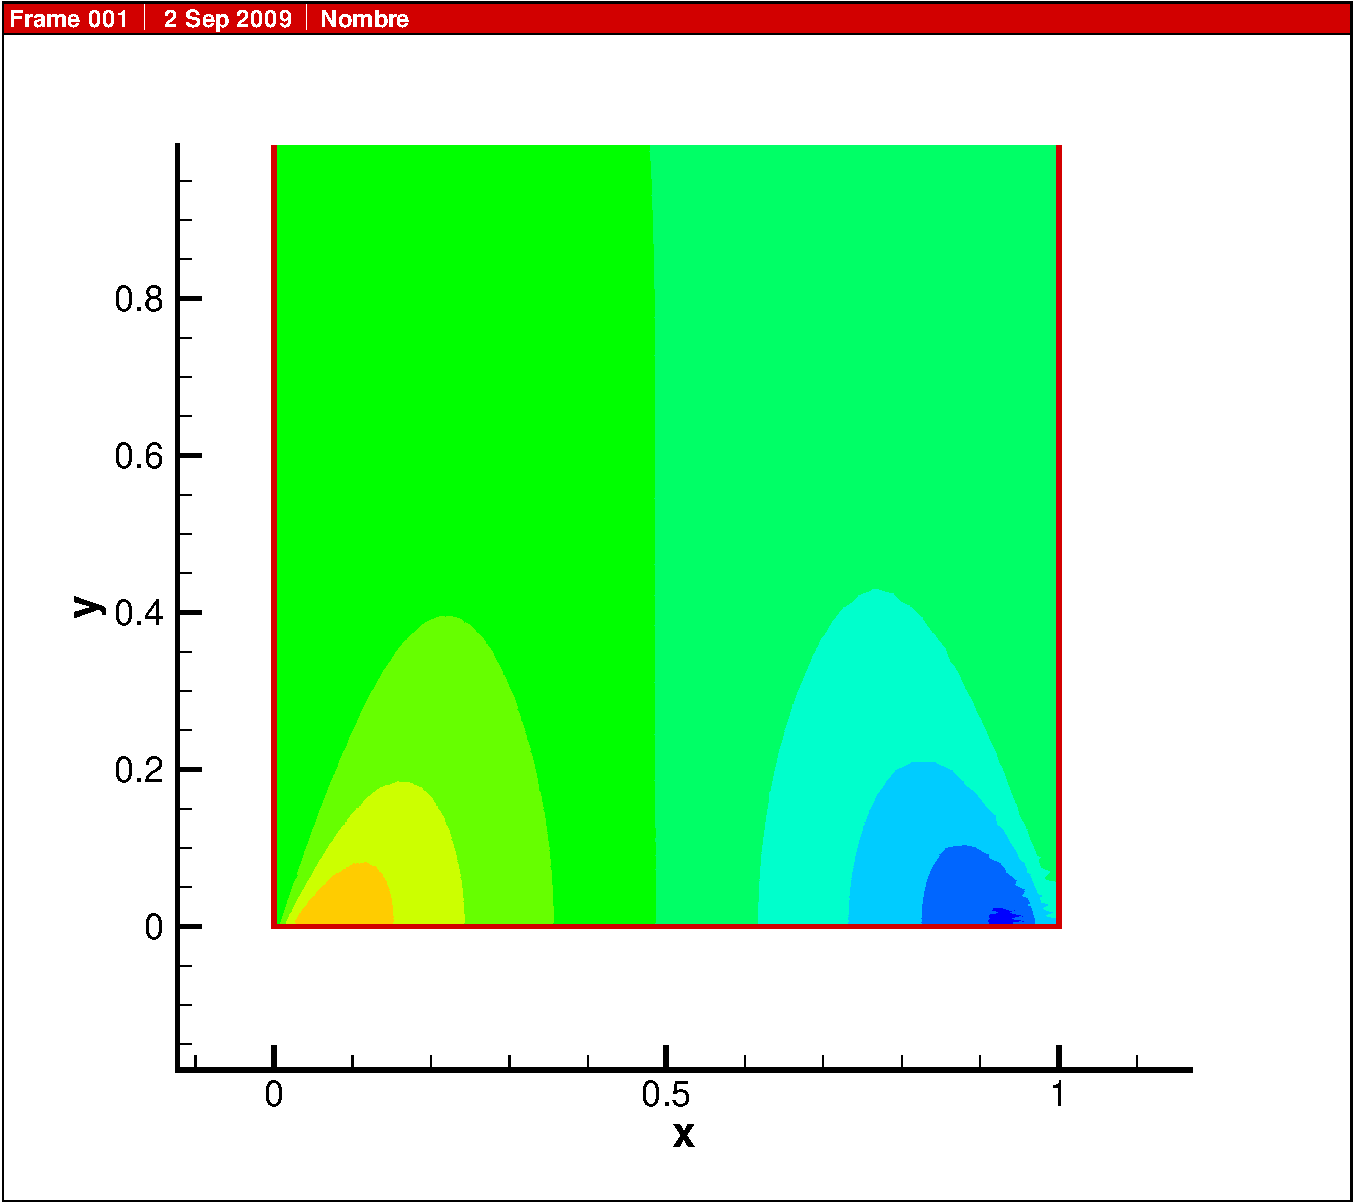
\includegraphics[width=\textwidth]{figs/LB-0-0-u-bas}
\caption{Level sets of horizontal velocity $U$ at the inlet using
  $U_{y} = 0$ and local Bernoulli, showing an aspiration.}
\label{fig:LB-0-0-u-bas}
\end{figure}


Using local or global boundary conditions for the inlet considerably
changes the mass flux, with higher fluxes for global Bernoulli. An
heuristic argument to explain this effect is as follows : global
Bernoulli, by increasing mean pressure, leads to higher vertical
velocities at the inlet. Indeed, mean pressure at the inlet using
global Bernoulli is $- \frac 1 2 (\int_{\text{inlet}} V)^{2}$, and with local
Bernoulli it is $- \frac 1 2 (\int_{\text{inlet}} V^{2})$. A simple
application of Cauchy-Schwartz inequality shows that mean pressure is
higher when using global Bernoulli. As a consequence, a surpression is
created, which increases velocities and reduces pressure. The
resulting profiles are given figures \ref{fig:GB-v} and \ref{fig:LB-pv}.

\begin{figure}[h!]
\centering
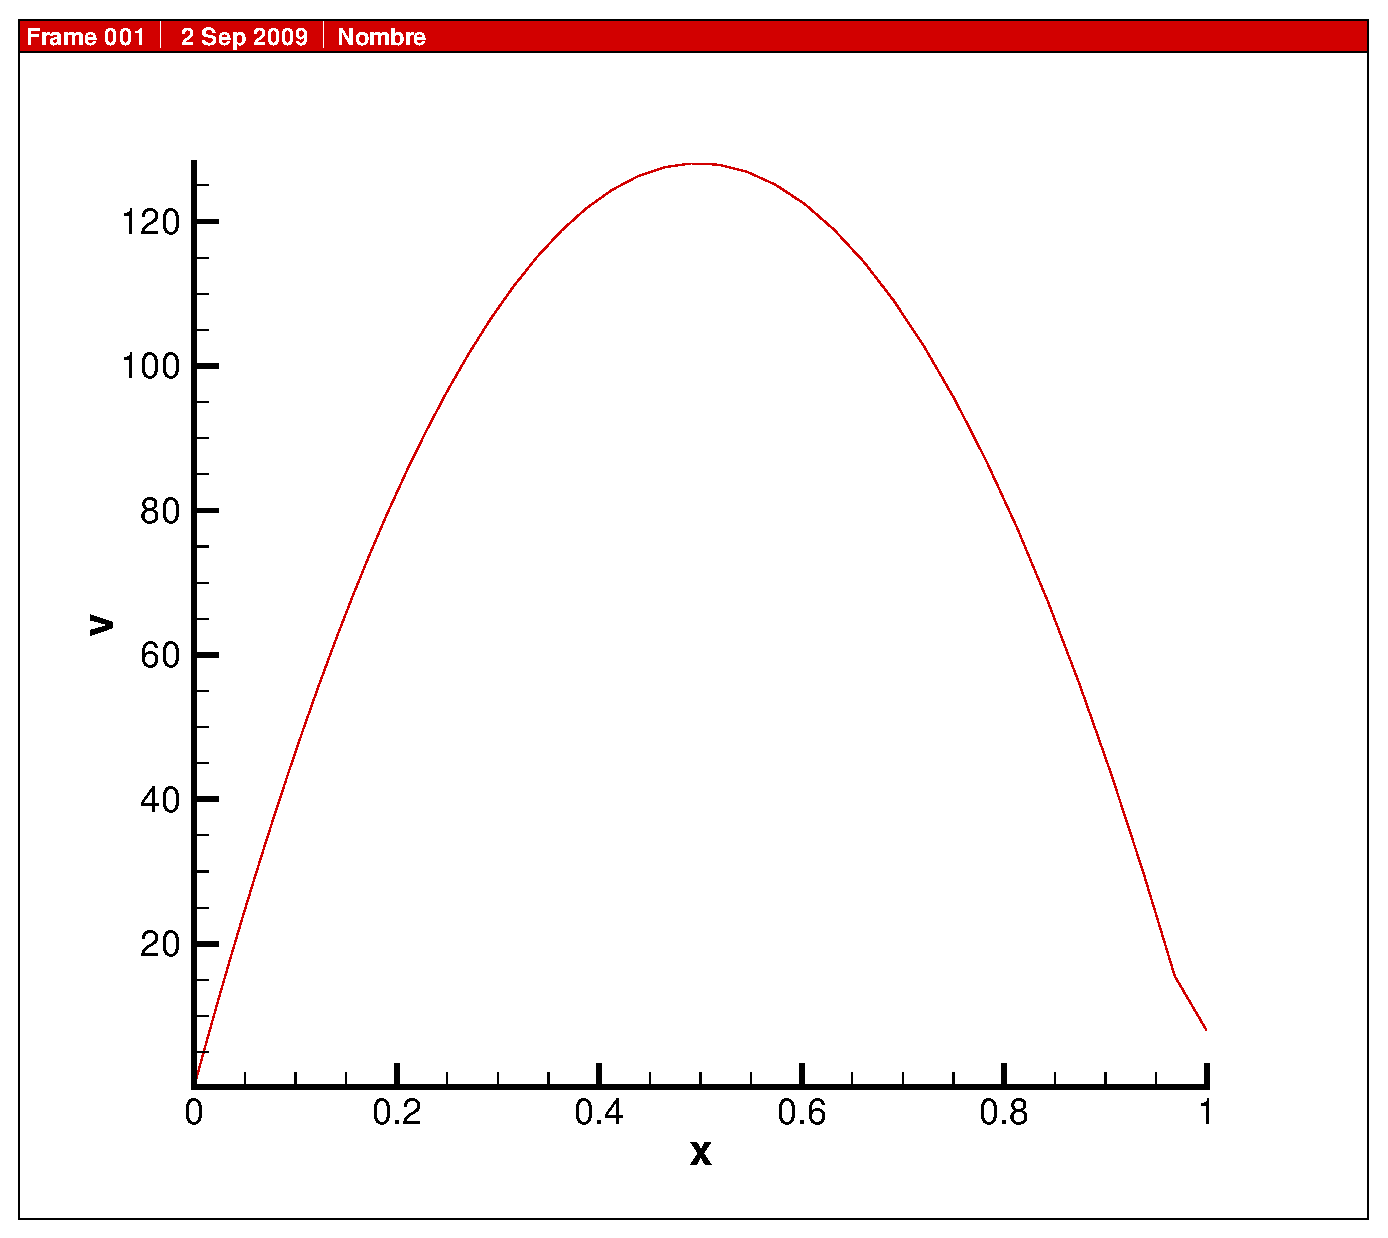
\includegraphics[width=0.6\textwidth]{figs/GB-v}
\caption{Vertical velocity profile at the inlet, for global
  Bernoulli. Pressure is -3660.}
\label{fig:GB-v}
\end{figure}

\begin{figure}[h!]
\centering
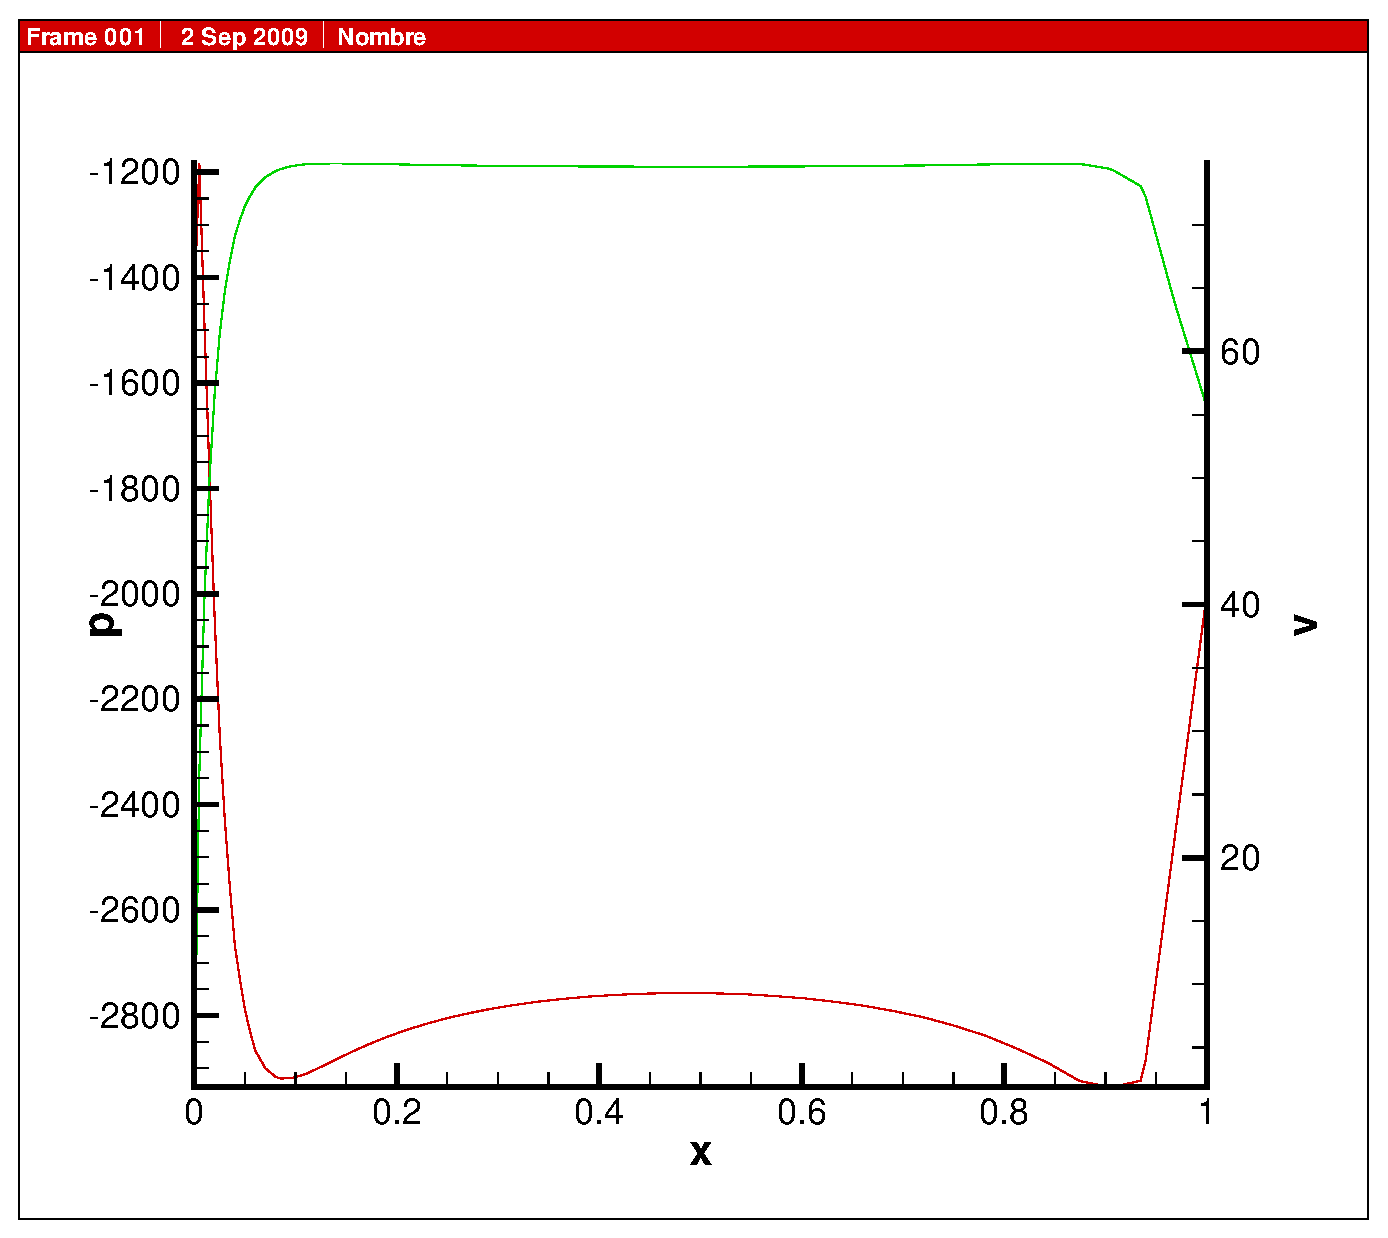
\includegraphics[width=0.6\textwidth]{figs/LB-pv}
\caption{Vertical velocity (top, right scale) and pressure (bottom,
  left scale) profile at the inlet, for local Bernoulli.}
\label{fig:LB-pv}
\end{figure}


\section{Conclusion}
TODOFIN

\listoffigures
\listoftables


\bibliographystyle{plain}
\addcontentsline{toc}{section}{References}
\bibliography{rapport}


\end{document}
